\documentclass[class=book, crop=false]{standalone}
\usepackage[subpreambles=true]{standalone}
\usepackage{import}
\usepackage[utf8]{inputenc}
\usepackage[margin=1.2in]{geometry}
\usepackage[sorting = none,
            doi = true  %lesedato for url-adresse
            ]{biblatex} %none gir bibliografi i sitert rekkefølge
\addbibresource{reference.bib}
\usepackage{csquotes}
\usepackage{float}


\begin{document}
\section{Programming software}
Python is the programming language used for this solving this task. Python is an open-source software that has several packages for machine learning and power flow calculations \cite{python_web}. In this thesis, \textit{pandapower} is the python package used for defining an electric power system and preforming power flow calculations\cite{pandapower}. \textit{Keras} is the Python package used for training a reinforcement agent \cite{keras_chollet2015}.

\section{Pandapower}
Pandapower is a time independent simulation tool, which means that it finds steady state solutions to a power flow problem. Consequently, the transitions from one state to another is not covered in this thesis.

This section will describe the different electrical elements available in pandapower and how they are physically modelled.
\subsection{Lines}
A line element can be added and connected between two buses by using the \texttt{pandapower.create\_line} method. Pandapower offers many standard types lines for both underground cables and overhead transmission lines. Alternatively a custom line can be specified with the method \texttt{pandapower.create\_line\_from\_parameters}. The line are modelled using the $\pi$-equivalent model, mentioned in section \ref{section:pi_model}.

\subsection{Generators}
Pandapower has two generator types. The first type is simply called generator and is modelled as a PV-bus. In other words, the active power production $P$ and voltage magnitude $|U|$ is are known when solving the power flow equations. Generators can be created using the method \texttt{pandapower.create\_gen}, where nominal values for apparent power and voltage can be specified. The second type is the static generator, where the active power $P$ and reactive power $Q$ is specified (PQ-bus). Static generators are created using \texttt{pandapower.create\_sgen}. Pandapower models power from the consumer perspective, so negative values for active power $P$ corresponds to generation of power.

\subsection{Loads}
The load in pandapower is modelled as a PQ-bus, where active and reactive power are known. Loads are created using the method \texttt{pandapower.create\_load}. The loads can also be modelled with constant impedance $Z$, current $I$ and $P$. In other words, replacing reactive power with current and impedance.

\subsection{Transformers}
Pandapower offers both two-winding and three-winding transformers that can be created from standard types using the \texttt{pandapower.create\_transformer} method, or from parameters using the method
\texttt{pandapower.create\_transformer\_from\_parameters}. The transformers can be modelled as a $\pi$-transformer or a $t$-transformer. The transformers can have settings for tap-position and phase-shifting of the voltage, which are a possible control variables for a reinforcement agent.  

\subsection{Storage}
It is possible to connect a storage element to a power grid using the \texttt{pandapower.create\_storage} method. The storage element is modelled as a PQ-node. Because simulations in pandapower is time-independent and only find steady state solution, it does not update the capacity of a storage during power flow calculations. Available energy in the storage element must therefore be updated manually according to some predefined timescale when several power flow calculations are performed.  


\section{Data structures in pandapower}

Pandapower stores information about elements in an electric transmission system in pandas DataFrames, which make it easy to inspect the numeric output of a power flow calculation. Figure \ref{fig:method:loading_example_net} shows a 4 bus case net and the components included in it. 

\begin{figure}[H]
    \center
    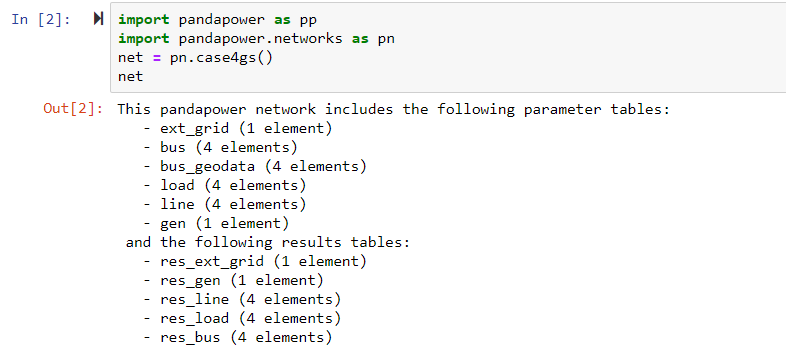
\includegraphics[height=6cm, width=12cm]{figures/case4g_show_net.PNG}
    \caption[size = 9]{Loading an example net in pandapower}
    \label{fig:method:loading_example_net}
\end{figure}
Each of the elements listed have a corresponding pandas DataFrame. The elements without "res" at the beginning are parameter tables and have information about nominal and max/min values for the components. Figure \ref{fig:method:line_bus_dataframe} shows the parameter table for the line and bus.

\begin{figure}[H]
    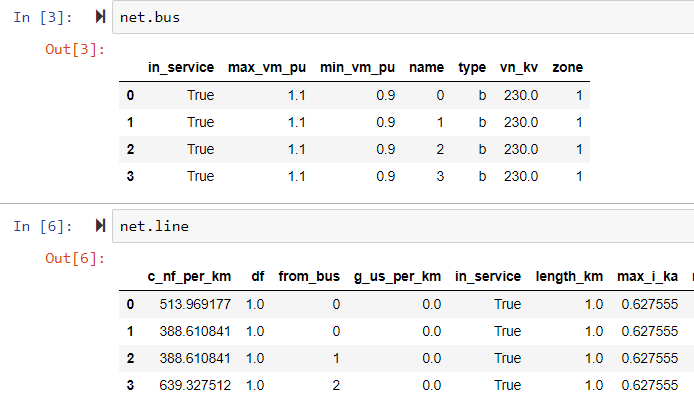
\includegraphics[height=7cm, width=13.5cm]{figures/case4g_line_bus.PNG}
    \caption[size = 9]{Parameter table in pandapower. There are more columns in net.line}
    \label{fig:method:line_bus_dataframe}
\end{figure}
All of the components will have a result table after the power flow calculation is performed, using the method \texttt{pandapower.runpp}. Figure \ref{fig:method:res_line_bus_dataframe} shows the result table for the bus and line.

\begin{figure}[H]
    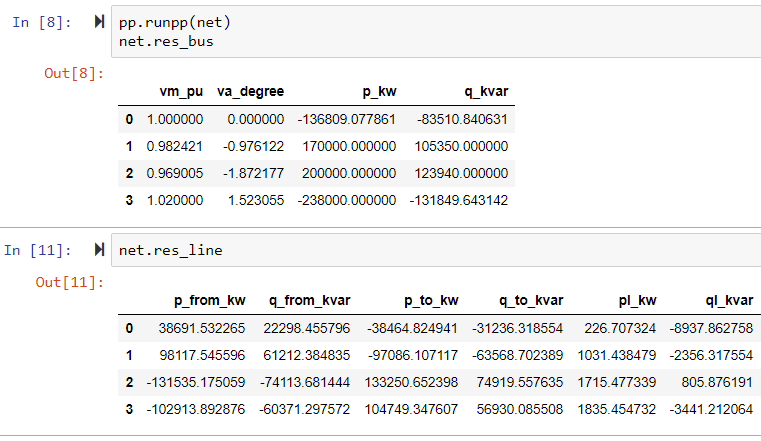
\includegraphics[height=8cm, width=14cm]{figures/case4g_line_bus_res.PNG}
    \caption[size = 9]{Result table in pandapower. There are more columns in net.res\_line}
    \label{fig:method:res_line_bus_dataframe}
\end{figure}

\section{Plotting results}
It is important to be able to inspect the resulting state after a reinforcement agent performs an action on the system. This can be complicated for large network with many buses and lines that each have a voltage magnitude, voltage angle and so on. Luckily, pandapower has support for plotting both grid architecture and results from the power flow. It is possible to get static plots using matplotlib and interactive plots using plotly\cite{plotly}. Figure \ref{fig:method:oberrhein_grid_results_plotly} shows the interactive results from a power flow calculation performed on the Oberrhein power grid using plotly. The lines are coloured based on the line loading (100\% means maximum current), while the buses are coloured based on the voltage magnitude. Such plots help to get a overview of the grid and quickly identify critical areas in the transmission system. Since the plot is interactive, it is easy to zoom and it is possible to click on a line or bus to see the relevant values. 


\begin{figure}[H]
    \center
    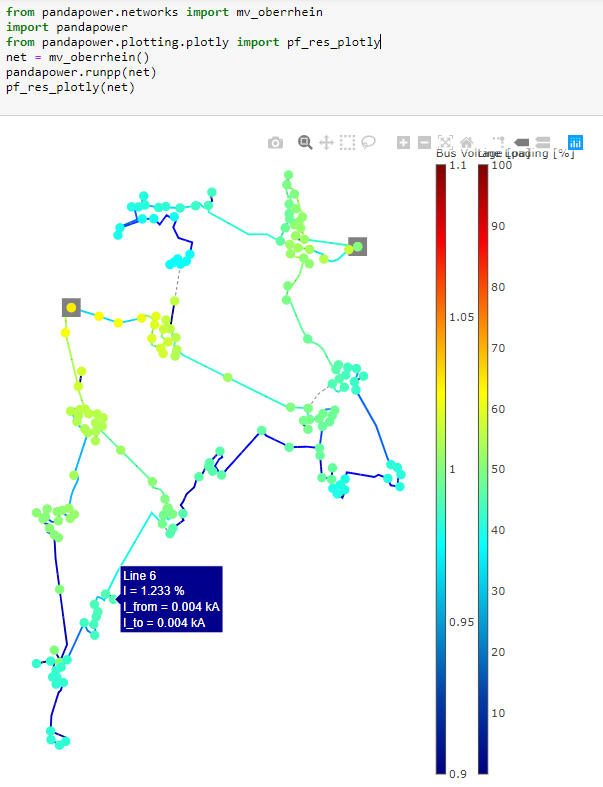
\includegraphics[height=13cm, width=12cm]{figures/results_pp_oberrhein.png}
    \caption[size = 9]{Interactive plot of the results from a power flow calculation on the Oberrhein case power grid using plotly. The grid consist of 179 lines and 180 buses}
    \label{fig:method:oberrhein_grid_results_plotly}
\end{figure}


\section{Controlling a pandapower net}
Reinforcement learning is all about taking actions and getting rewards based on how good that action was. It must therefore be possible to control certain elements in a pandapower net. This section will show how to perform certain actions in pandapowers. \texttt{net.gen} gives a DataFrame where all the generators in the system is represented as a row. Because a generator is modelled as a PV-bus, it is possible to control the voltage and power by overwriting the parameters in \texttt{net.gen}. Figure \ref{fig:method:case4g_controll_vm_p_kw} shows how to set the active power production to 100000 kW and voltage magnitude to 0.99. The last row in the \texttt{net.res\_bus} is the bus where the generator is connected, and we see that the voltage magnitude is the same as the generator voltage magnitude. The power production if different from 100000 kW because there is a 80000 kW load connected to the same bus, and the table shows the sum of production and consumption at each bus. 



\begin{figure}[H]
    \center
    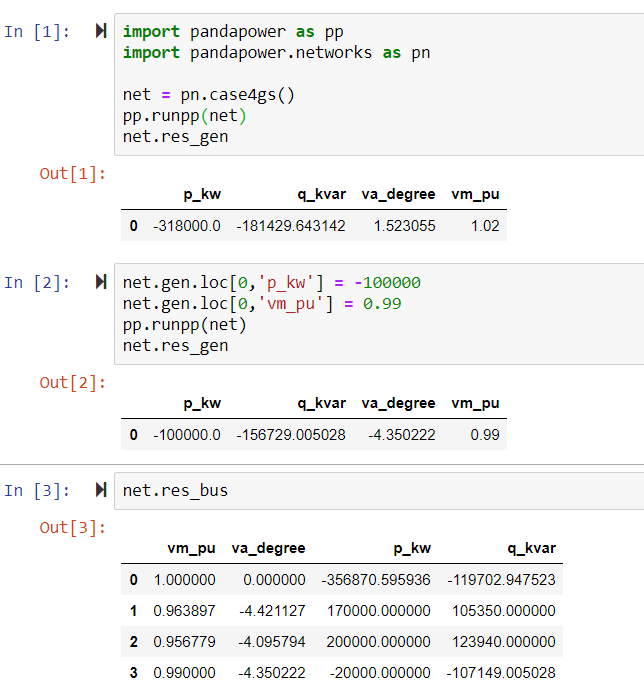
\includegraphics[height=12cm, width=12cm]{figures/case4g_controll_vm_p_kw.PNG}
    \caption[size = 9]{How to control the active power and voltage magnitude at a generator. Note that negative values for active power ('p\_kw') means production}
    \label{fig:method:case4g_controll_vm_p_kw}
\end{figure}

Transformers in a transmission system can have controllable taps that change the winding ratio between the low and high voltage side of the transformer. By doing this it is possible to control the voltage magnitude at buses connected to a transformer. There also exists phase-shifting transformers that can manipulate the the voltage angle between the low and high voltage side. Transformers in pandapower allow control of both voltage magnitude $|U|$ and voltage angle $\delta$. The code in figure \ref{fig:method:control_transformer} demonstrates how to control a transformer in pandapower. First, a two bus system with a transformer is created. It is a standard type transformer 25 MVA, 110/20 kV and the external grid is connected to the high voltage side of the transformer. The taps are placed on the low voltage side of the transformer with the command \texttt{net.trafo['tp\_side'] = 'lv'}. Performing a power flow calculation gives the result tables without changing the tap position in the transformer. The voltage angle is manipulated to 20 degrees by specifying \texttt{net.trafo['shift\_degree']}. The voltage magnitude is changed by first specifying \texttt{net.trafo['tp\_st\_percent']} which is the percentage change in voltage magnitude per tap position. This is set to 10 \% and the tap position is set using \texttt{net.trafo['tp\_pos']} to -1. By running another power flow calculation and inspecting the table \texttt{net.res\_bus}, it is evident that the voltage angle is shifted 20 degrees and that the voltage magnitude is reduced by 10 \% with respect to the first power flow calculation. 


\begin{figure}[H]
    \center
    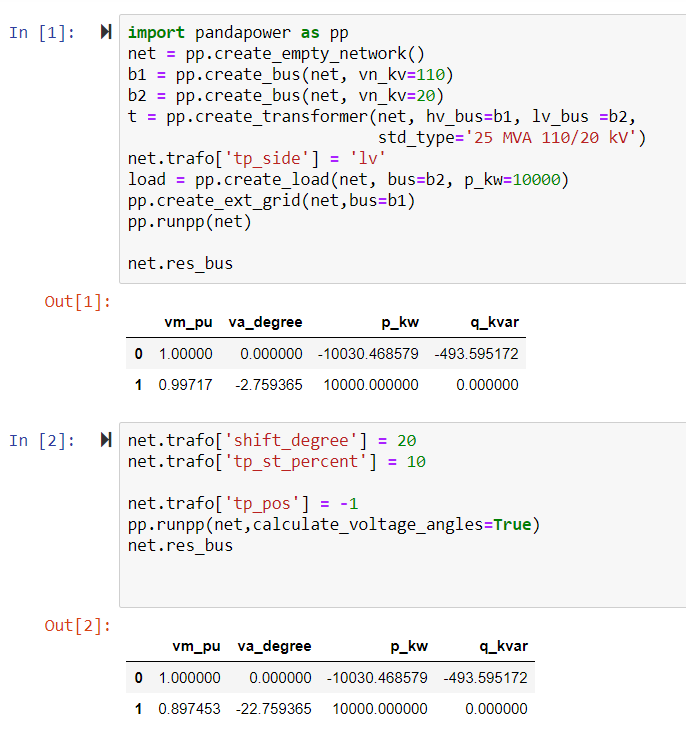
\includegraphics[height=12cm, width=12cm]{figures/control_transformer.PNG}
    \caption[size = 9]{Code of of to control the tap position and phase angle for a transformer in pandapower}
    \label{fig:method:control_transformer}
\end{figure}






\end{document}

